\chapter{Titrasi dengan pH dan Konduktivitas}\label{ch:g12:ph-conductivity-titrations}

Sebotol cuka anggur berlabel ``keasaman 6 \%'': enam gram asam etanoat
dalam setiap seratus gram cuka. Baik asam etanoat maupun basa
konjugatnya tidak berwarna, dan permanganat tidak dapat membantu di
sini. Tetapi \omterm{def:g9:acids-bases-ph:ph-paper}{pH meter} yang dicelupkan ke dalam cuka itu, atau sebuah sel
yang mengukur seberapa baik cuka itu menghantarkan listrik, mengikuti
reaksinya dengan basa tetes demi tetes, dan bentuk kurvanya
memperlihatkan dengan tepat di mana \omterm{def:g11:titration:equivalence}{titik ekuivalennya}. Sepuluh menit di
meja laboratorium, dan labelnya pun terperiksa.

\begin{recall}
\omterm{def:g11:titration:titration}{Titrasi}, \omterm{def:g11:titration:equivalence}{titik ekuivalen} dan \omterm{def:g11:titration:equivalence}{volume ekuivalennya}
(\cref{ch:g11:titration}); \omterm{def:g12:ka-and-pka:ka}{tetapan keasaman} (\cref{ch:g12:ka-and-pka});
hubungan Henderson dan indikator
(\cref{ch:g12:buffers-predominance}); larutan \omterm{def:g9:ions:ion}{ion} menghantarkan listrik
(\cref{ch:g9:ions}).
\end{recall}

\begin{omfigure}
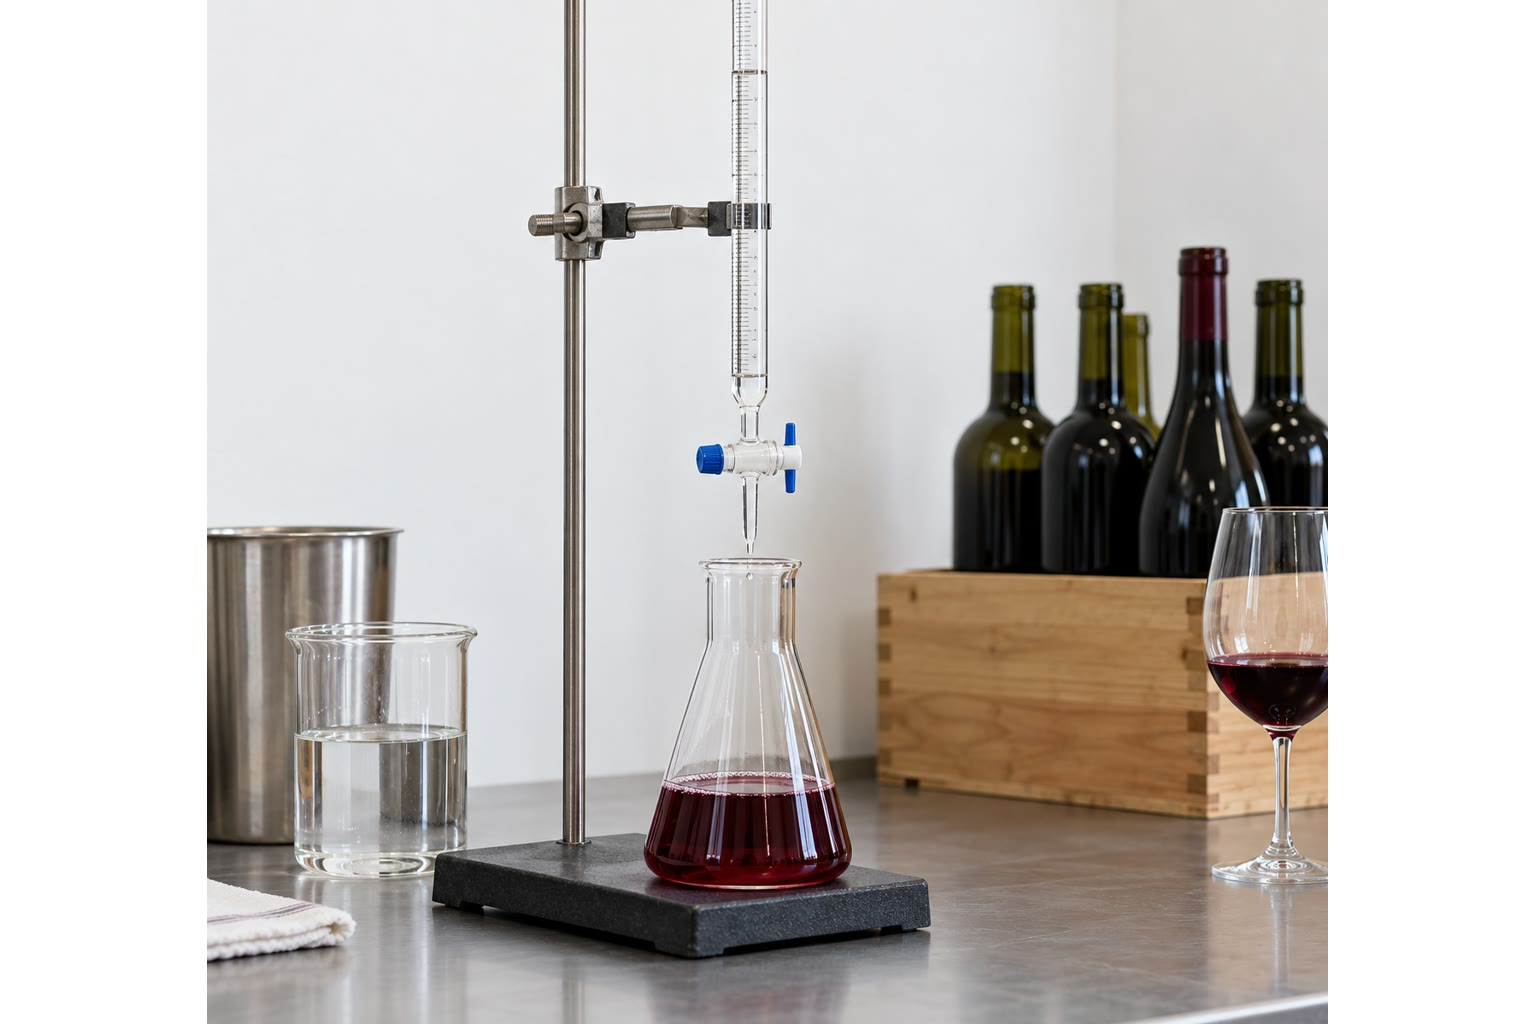
\includegraphics[width=0.45\linewidth]{images/book1/ai/g12-wine-lab.jpg}

{\small Meja \omterm{def:g11:titration:titration}{titrasi} seorang pembuat anggur.}
\end{omfigure}

\section{Titrasi pH-metri}

\begin{definition}[Titrasi pH-metri, setengah ekuivalen]\label{def:g12:ph-conductivity-titrations:ph-metric}
Dalam \emph{titrasi pH-metri}\index{titrasi pH-metri}, \omterm{def:g9:acids-bases-ph:ph}{pH} \omterm{def:g11:titration:titration}{larutan yang
dititrasi} diukur setelah setiap penambahan \omterm{def:g11:titration:titration}{titran}, lalu kurva \omterm{def:g9:acids-bases-ph:ph}{pH}
terhadap volume yang ditambahkan digambar. Yang disebut
\emph{setengah ekuivalen}\index{setengah ekuivalen} adalah titik saat
setengah \omterm{def:g11:titration:equivalence}{volume ekuivalen} telah ditambahkan.
\end{definition}

\begin{omfigure}
\begin{tikzpicture}[font=\small, scale=0.65]
  \pic[transform shape] at (0,0) {stand={6.3}{2.0}};
  \pic[transform shape] at (2.0,0.68) {stirrer};
  \pic[transform shape] at (2.0,0.68) {beaker={0.45}{omWater}};
  \pic[transform shape] at (2.0,2.9) {burette={0.8}{omWater}};
  \pic[transform shape] (pr) at (2.6,0.95) {probe};
  \pic[transform shape] (m) at (6.4,3.4) {meter={pH}};
  \draw[black!70, thick] (pr-top) .. controls +(0,1.0) and +(0,-1.2) .. (m-a);
  \draw[omProp, thick, <-] (2.35,7.2) -- (4.3,7.6) node[right, text=black] {buret: NaOH};
  \draw[omProp, thick, <-] (1.4,1.1) -- (-1.4,1.6) node[left, text=black, align=right] {asam yang dititrasi};
  \draw[omProp, thick, <-] (2.75,2.4) -- (4.3,2.0) node[right, text=black] {elektrode pH};
\end{tikzpicture}

{\small \omterm{def:g12:ph-conductivity-titrations:ph-metric}{Titrasi pH-metri}: elektrodenya tercelup dalam larutan yang
diaduk, dan alat ukurnya menunjukkan \omterm{def:g9:acids-bases-ph:ph}{pH} setelah setiap penambahan.}
\end{omfigure}

\begin{inthelab}[Mengalibrasi pH meter]
Sebelum dipakai, elektrodenya dibilas dengan air suling dan dicelupkan
ke dalam dua \omterm{def:g12:buffers-predominance:buffer}{larutan penyangga} yang \omterm{def:g9:acids-bases-ph:ph}{pH-nya} diketahui, biasanya 7.0 dan
4.0 (atau 10.0): alat ukurnya diatur agar menunjukkan nilai-nilai itu.
Di antara larutan-larutan itu elektrodenya dibilas dan ditepuk-tepuk
kering dengan lembut, tidak pernah digosok; elektrode disimpan dengan
ujungnya tetap basah.
\end{inthelab}

\begin{omfigure}
\begin{minipage}{0.49\linewidth}
\begin{tikzpicture}
\begin{axis}[width=\linewidth, height=6cm, xmin=0, xmax=30, ymin=0, ymax=14,
    xlabel={$V_{\text{NaOH}}$ (\si{mL})}, ylabel={pH}, axis lines*=left,
    ymajorgrids, grid style={gray!20}, tick label style={font=\scriptsize},
    label style={font=\small}, title={\small \ce{HCl} oleh \ce{NaOH}},
    title style={yshift=-4pt}]
  \addplot[very thick, omDef] table[x=V, y=pH] {figdata/out/grade-12-ph-conductivity-titrations-a.dat};
  \addplot[thick, omProp, densely dotted] table[x=V, y expr=\thisrow{dpH}/4]
    {figdata/out/grade-12-ph-conductivity-titrations-a.dat};
  \addplot[dashed, black!60] coordinates {(20,0) (20,7)};
  \node[font=\scriptsize, anchor=north west] at (axis cs:20.3,6.5) {$V_E = 20.0$};
\end{axis}
\end{tikzpicture}
\end{minipage}\hfill
\begin{minipage}{0.49\linewidth}
\begin{tikzpicture}
\begin{axis}[width=\linewidth, height=6cm, xmin=0, xmax=16, ymin=0, ymax=14,
    xlabel={$V_{\text{NaOH}}$ (\si{mL})}, ylabel={pH}, axis lines*=left,
    ymajorgrids, grid style={gray!20}, tick label style={font=\scriptsize},
    label style={font=\small}, title={\small \ce{CH3COOH} oleh \ce{NaOH}},
    title style={yshift=-4pt}]
  \addplot[very thick, omDef] table[x=V, y=pH] {figdata/out/grade-12-ph-conductivity-titrations-b.dat};
  \addplot[thick, omProp, densely dotted] table[x=V, y expr=\thisrow{dpH}/4]
    {figdata/out/grade-12-ph-conductivity-titrations-b.dat};
  \addplot[dashed, black!60] coordinates {(10.1,0) (10.1,8.7)};
  \addplot[dashed, black!60] coordinates {(0,4.76) (5.05,4.76) (5.05,0)};
  \node[font=\scriptsize, anchor=south west] at (axis cs:0.2,4.8) {$pK_a = 4.76$};
  \node[font=\scriptsize, anchor=north west] at (axis cs:10.4,3.0) {$V_E = 10.1$};
\end{axis}
\end{tikzpicture}
\end{minipage}

{\small Kurva \omterm{def:g9:acids-bases-ph:ph}{pH} hasil perhitungan (biru) dan turunannya
$d\mathrm{pH}/dV$ (jingga, bertitik, dibagi 4). Kiri: \qty{20.0}{mL}
asam klorida \qty{0.100}{mol/L}; \omterm{def:g11:titration:equivalence}{titik ekuivalen} pada \omterm{def:g9:acids-bases-ph:ph}{pH} 7.00. Kanan:
\qty{10.0}{mL} cuka yang diencerkan; pada \omterm{def:g12:ph-conductivity-titrations:ph-metric}{setengah ekuivalen} \omterm{def:g9:acids-bases-ph:ph}{pH} sama
dengan $pK_a$, dan \omterm{def:g11:titration:equivalence}{titik ekuivalennya} berada pada \omterm{def:g9:acids-bases-ph:ph}{pH} basa.}
\end{omfigure}


\begin{method}[Metode turunan]\label{met:g12:ph-conductivity-titrations:derivative}
Hitung, di antara pengukuran-pengukuran yang berurutan, kemiringan
$\Delta\mathrm{pH}/\Delta V$, lalu gambarlah grafiknya terhadap $V$
(lembar kerja atau kalkulator dapat melakukannya). \omterm{def:g11:titration:equivalence}{Volume ekuivalen}
terletak di tempat kemiringan ini paling besar: puncak kurva turunannya.
\end{method}

\begin{method}[Metode garis singgung]\label{met:g12:ph-conductivity-titrations:tangent}
\begin{enumerate}
  \item Gambarlah dua garis singgung yang sejajar pada kurva, satu
        sebelum lonjakan dan satu sesudahnya, di kedua sisinya.
  \item Gambarlah garis sejajar yang terletak tepat di tengah keduanya.
  \item Titik potongnya dengan kurva adalah \omterm{def:g11:titration:equivalence}{titik ekuivalen}: bacalah
        $V_E$ (dan \omterm{def:g9:acids-bases-ph:ph}{pH} pada \omterm{def:g11:titration:equivalence}{titik ekuivalen}).
\end{enumerate}
\end{method}

\begin{proposition}[Pada setengah ekuivalen, $\mathrm{pH} = pK_a$]\label{prop:g12:ph-conductivity-titrations:half}
Pada \omterm{def:g11:titration:titration}{titrasi} \omterm{def:g12:ka-and-pka:strong-acid}{asam lemah} \ce{HA} dengan \omterm{def:g12:ka-and-pka:strong-acid}{basa kuat}, pada \omterm{def:g12:ph-conductivity-titrations:ph-metric}{setengah
ekuivalen} $\mathrm{pH} = pK_a$.
\end{proposition}

\begin{proof}
Reaksi \ce{HA + OH- -> A- + H2O} berlangsung tuntas. Pada \omterm{def:g12:ph-conductivity-titrations:ph-metric}{setengah
ekuivalen}, setengah dari asamnya telah berubah menjadi \ce{A-}:
$[\ce{A-}] = [\ce{HA}]$, dan hubungan Henderson memberikan
$\mathrm{pH} = pK_a + \log 1 = pK_a$.
\end{proof}

\begin{remark}[Memilih indikator dari kurva]\label{rem:g12:ph-conductivity-titrations:indicator}
% ledger: ind:BBT, ind:phenolphthalein
Indikator harus berubah warna di dalam lonjakan. Untuk asam klorida,
lonjakannya membentang dari sekitar \omterm{def:g9:acids-bases-ph:ph}{pH} 4 sampai 10 dan banyak indikator
yang cocok, terutama biru bromtimol; untuk asam etanoat, lonjakannya
lebih pendek dan bersifat basa, sekitar 7 sampai 11: fenolftalein
(8.0--10.0) cocok, sedangkan biru bromtimol akan berubah terlalu cepat.
\end{remark}

\section{Konduktivitas dan titrasi konduktometri}

\begin{definition}[Konduktivitas, konduktivitas ionik molar]\label{def:g12:ph-conductivity-titrations:conductivity}
Besaran yang disebut \emph{konduktivitas}\index{konduktivitas} $\sigma$ sebuah
larutan mengukur seberapa baik larutan itu menghantarkan listrik;
nilainya dibaca pada konduktometer dalam \si{mS/cm} (atau \si{S/m}).
Setiap \omterm{def:g9:ions:ion}{ion} $i$ menyumbang padanya sebanding dengan konsentrasinya,
dengan sebuah koefisien $\lambda_i$, yaitu
\emph{konduktivitas ionik molar}\index{konduktivitas ionik molar}-nya.
\end{definition}

\begin{proposition}[Hukum Kohlrausch]\label{prop:g12:ph-conductivity-titrations:kohlrausch}
% ledger: lam:H+, lam:OH-, lam:Na+, lam:Cl-
Untuk larutan encer, $\sigma = \sum_i \lambda_i [X_i]$. Pada
\qty{25}{\celsius}, dalam \si{S.cm^2/mol}: \ce{H3O+} 349.8, \ce{OH-}
198.3, \ce{Cl-} 76.2, \ce{Na+} 50.3. \omterm{def:g12:ka-and-pka:oxonium}{Ion oksonium} dan \omterm{def:g9:ions:ion}{ion} hidroksida
menghantarkan listrik jauh lebih baik daripada semua \omterm{def:g9:ions:ion}{ion} lain.
\end{proposition}

\begin{proof}
Diterima tanpa bukti (buku Tahun Pertama universitas). Nilai \ce{Cl-}
dan \ce{Na+} berasal dari \omterm{def:g12:ph-conductivity-titrations:conductivity}{konduktivitas} terukur larutan asam klorida dan
natrium klorida, yang dikurangi dengan nilai \ce{H3O+}.
\end{proof}

\begin{definition}[Titrasi konduktometri]\label{def:g12:ph-conductivity-titrations:conductimetric}
Dalam \emph{titrasi konduktometri}\index{titrasi konduktometri},
\omterm{def:g12:ph-conductivity-titrations:conductivity}{konduktivitas} diukur setelah setiap penambahan \omterm{def:g11:titration:titration}{titran}. \omterm{def:g11:titration:titration}{Larutan yang
dititrasi} diencerkan dalam air yang banyak, sehingga volume yang
ditambahkan hampir tidak mengubahnya: titik-titiknya lalu terletak pada
garis-garis lurus, yang berubah kemiringannya pada \omterm{def:g11:titration:equivalence}{titik ekuivalen}.
\end{definition}

\begin{omfigure}
\begin{minipage}{0.4\linewidth}\centering
\begin{tikzpicture}[font=\small, scale=0.75]
  \pic[transform shape] at (0,0) {beaker={0.6}{omWater}};
  \pic[transform shape] (cc) at (0.2,0.2) {condcell};
  \pic[transform shape] (m) at (2.6,3.4) {meter={mS/cm}};
  \draw[black!70, thick] (cc-top) .. controls +(0,0.8) and +(0,-1) .. (m-a);
  \node[anchor=north, align=center] at (0.6,-0.15) {sel konduktometri\\ di dalam larutan};
\end{tikzpicture}
\end{minipage}\hfill
\begin{minipage}{0.56\linewidth}
\begin{tikzpicture}
\begin{axis}[width=\linewidth, height=5.4cm, xmin=0, xmax=20, ymin=0,
    ymax=4.6, xlabel={$V_{\text{NaOH}}$ (\si{mL})}, ylabel={$\sigma$ (\si{mS/cm})},
    axis lines*=left, ymajorgrids, grid style={gray!20},
    tick label style={font=\scriptsize}, label style={font=\small}]
  \addplot[only marks, mark=*, mark size=1.4pt, omDef] table[x=V, y=sigma]
    {figdata/out/grade-12-ph-conductivity-titrations-c.dat};
  \addplot[dashed, black!60] coordinates {(10,0) (10,4.6)};
  \node[font=\scriptsize, anchor=south west] at (axis cs:10.3,0.2) {$V_E = 10.0$};
\end{axis}
\end{tikzpicture}
\end{minipage}

{\small Kiri: sel konduktometri. Kanan: \qty{100}{mL} asam klorida
\qty{0.0100}{mol/L} yang dititrasi dengan natrium hidroksida
\qty{0.100}{mol/L} (dihitung dengan hukum Kohlrausch). \omterm{def:g12:ph-conductivity-titrations:conductivity}{Konduktivitasnya}
turun, lalu naik: dua garis lurus yang bertemu pada \omterm{def:g11:titration:equivalence}{titik ekuivalen}.}
\end{omfigure}

\begin{example}[Membaca kedua garis]\label{ex:g12:ph-conductivity-titrations:lines}
Sebelum \omterm{def:g11:titration:equivalence}{titik ekuivalen}, setiap \ce{OH-} yang ditambahkan menyingkirkan
sebuah \ce{H3O+} ($\lambda = 349.8$) dan membawa masuk sebuah \ce{Na+}
($\lambda = 50.3$): \omterm{def:g12:ph-conductivity-titrations:conductivity}{konduktivitasnya} turun tajam. Sesudah \omterm{def:g11:titration:equivalence}{titik
ekuivalen}, \ce{Na+} dan \ce{OH-} ($\lambda = 198.3$) hanya menumpuk:
\omterm{def:g12:ph-conductivity-titrations:conductivity}{konduktivitasnya} naik. Kedua garis bertemu pada
$V_E = \qty{10.0}{mL}$, jadi konsentrasi asamnya
$0.100 \times 10.0 / 100 = \qty{0.0100}{mol/L}$.
\end{example}

\begin{method}[Titik ekuivalen dari titrasi konduktometri]\label{met:g12:ph-conductivity-titrations:two-lines}
Gambarlah garis lurus terbaik melalui titik-titik sebelum \omterm{def:g11:titration:equivalence}{titik
ekuivalen} dan garis terbaik melalui titik-titik sesudahnya; bacalah
$V_E$ pada perpotongannya. Titik-titik di dekat \omterm{def:g11:titration:equivalence}{titik ekuivalen}, tempat
garis-garisnya melengkung, tidak dipakai.
\end{method}

\begin{remark}[Metode mana, kapan]\label{rem:g12:ph-conductivity-titrations:which}
Indikator berwarna paling cepat jika ada indikator yang cocok. \omterm{def:g12:ph-conductivity-titrations:ph-metric}{Titrasi
pH-metri} juga memberikan $pK_a$ \omterm{def:g12:ka-and-pka:strong-acid}{asam lemah}, dan dapat dipakai untuk
larutan yang berwarna atau keruh. \omterm{def:g12:ph-conductivity-titrations:conductimetric}{Titrasi konduktometri} sama sekali
tidak memerlukan lonjakan \omterm{def:g9:acids-bases-ph:ph}{pH}: \omterm{def:g11:titration:titration}{titrasi} ini dapat dipakai untuk asam yang
sangat lemah atau sangat encer, dan untuk \omterm{def:g9:ions:precipitate}{reaksi pengendapan}, selama
\omterm{def:g9:ions:ion}{ion-ionnya} berubah.
\end{remark}

\begin{safety}{\ghs[0.82cm]{GHS05}\ghs[0.82cm]{GHS07}}
% ledger: ghs:NaOH
Larutan natrium hidroksida membakar kulit dan mata, bahkan larutan encer
jika mengenai mata: pakailah kacamata pelindung sepanjang waktu, dan
setiap percikan segera dibilas dengan banyak air.
\end{safety}

\section{Latihan}


\begin{exercise}[$\star$]\label{exo:g12:ph-conductivity-titrations:1}
Bacalah \omterm{def:g11:titration:equivalence}{volume ekuivalen} pada kurva asam klorida yang dititrasi dengan
natrium hidroksida \qty{0.100}{mol/L}, lalu simpulkan konsentrasi
\qty{20.0}{mL} asam itu.
\end{exercise}

\begin{exercise}[$\star$]\label{exo:g12:ph-conductivity-titrations:2}
Sebuah \omterm{def:g12:ka-and-pka:strong-acid}{asam lemah} dititrasi dengan natrium hidroksida;
$V_E = \qty{12.0}{mL}$. Pada \qty{6.0}{mL}, \omterm{def:g9:acids-bases-ph:ph}{pH-nya} 3.75. Berikan
$pK_a$ asam itu. Asam mana pada skala $pK_a$ yang mungkin?
\end{exercise}

\begin{exercise}[$\star$]\label{exo:g12:ph-conductivity-titrations:3}
Indikator mana yang akan kamu pilih untuk \omterm{def:g11:titration:titration}{titrasi} asam etanoat dengan
natrium hidroksida? Mengapa bukan merah metil?
\end{exercise}

\begin{exercise}[$\star$]\label{exo:g12:ph-conductivity-titrations:4}
Mengapa \omterm{def:g9:acids-bases-ph:ph-paper}{pH meter} harus dikalibrasi sebelum dipakai? Dengan apa?
\end{exercise}

\begin{exercise}[$\star$]\label{exo:g12:ph-conductivity-titrations:5}
Dengan \omterm{def:g12:ph-conductivity-titrations:conductivity}{konduktivitas ionik molar}, urutkan \omterm{def:g9:ions:ion}{ion} \ce{H3O+}, \ce{OH-},
\ce{Na+}, \ce{Cl-} dari penghantar terbaik sampai yang terburuk.
\end{exercise}

\begin{exercise}[$\star\star$]\label{exo:g12:ph-conductivity-titrations:6}
Sebanyak \qty{20.0}{mL} larutan asam etanoat memerlukan \qty{14.6}{mL}
natrium hidroksida \qty{0.050}{mol/L}. Hitung konsentrasinya.
\end{exercise}

\begin{exercise}[$\star\star$]\label{exo:g12:ph-conductivity-titrations:7}
Di dekat \omterm{def:g11:titration:equivalence}{titik ekuivalen}, hasil pembacaannya: \qty{9.6}{mL}, \omterm{def:g9:acids-bases-ph:ph}{pH} 5.7;
\qty{9.8}{mL}, 6.1; \qty{10.0}{mL}, 7.0; \qty{10.2}{mL}, 10.5;
\qty{10.4}{mL}, 11.0. Hitung $\Delta\mathrm{pH}/\Delta V$ di antara
titik-titik yang berurutan, lalu tentukan letak $V_E$.
\end{exercise}

\begin{exercise}[$\star\star$]\label{exo:g12:ph-conductivity-titrations:8}
Pada \omterm{def:g12:ph-conductivity-titrations:conductimetric}{titrasi konduktometri} asam klorida, jelaskan tanda kemiringan
sebelum dan sesudah \omterm{def:g11:titration:equivalence}{titik ekuivalen}, dengan memakai \omterm{def:g9:ions:ion}{ion-ion} yang ada.
\end{exercise}

\begin{exercise}[$\star\star$]\label{exo:g12:ph-conductivity-titrations:9}
Sketsalah kurva konduktometri asam etanoat yang dititrasi dengan
natrium hidroksida. Mengapa \omterm{def:g12:ph-conductivity-titrations:conductivity}{konduktivitasnya} naik bahkan sebelum \omterm{def:g11:titration:equivalence}{titik
ekuivalen}?
\end{exercise}

\begin{exercise}[$\star\star$]\label{exo:g12:ph-conductivity-titrations:10}
Pada kurva hasil perhitungan untuk cuka yang diencerkan, bacalah \omterm{def:g9:acids-bases-ph:ph}{pH} di
awal, pada \omterm{def:g12:ph-conductivity-titrations:ph-metric}{setengah ekuivalen}, dan pada \omterm{def:g11:titration:equivalence}{titik ekuivalen}. Mengapa \omterm{def:g9:acids-bases-ph:ph}{pH}
awalnya jauh lebih tinggi daripada \omterm{def:g9:acids-bases-ph:ph}{pH} asam klorida dengan konsentrasi
yang sama?
\end{exercise}

\begin{exercise}[$\star\star$]\label{exo:g12:ph-conductivity-titrations:11}
Mengapa \omterm{def:g11:titration:titration}{larutan yang dititrasi} diencerkan dalam air yang banyak sebelum
\omterm{def:g12:ph-conductivity-titrations:conductimetric}{titrasi konduktometri}?
\end{exercise}

\begin{exercise}[$\star\star\star$]\label{exo:g12:ph-conductivity-titrations:12}
Sebuah larutan mengandung asam klorida sekaligus asam etanoat. Larutan
itu dititrasi dengan natrium hidroksida sambil \omterm{def:g9:acids-bases-ph:ph}{pH-nya} diukur. Jelaskan
mengapa kurvanya memperlihatkan dua lonjakan, dan apa yang diukur oleh
setiap \omterm{def:g11:titration:equivalence}{volume ekuivalen}.
\end{exercise}

\begin{exercise}[$\star\star\star$]\label{exo:g12:ph-conductivity-titrations:13}
Hitung \omterm{def:g12:ph-conductivity-titrations:conductivity}{konduktivitas} di awal \omterm{def:g12:ph-conductivity-titrations:conductimetric}{titrasi konduktometri} dalam bab ini (asam
klorida \qty{0.0100}{mol/L}) dan pada \omterm{def:g11:titration:equivalence}{titik ekuivalen} (\qty{110}{mL}
larutan natrium klorida). Bandingkan dengan gambar.
\end{exercise}

\begin{exercise}[$\star\star\star$]\label{exo:g12:ph-conductivity-titrations:14}
Sebuah \omterm{def:g9:acids-bases-ph:ph-paper}{pH meter} yang dikalibrasi dengan buruk menunjukkan setiap \omterm{def:g9:acids-bases-ph:ph}{pH} 0.2
terlalu tinggi. Kesalahan apa yang ditimbulkannya pada \omterm{def:g11:titration:equivalence}{volume ekuivalen}
\omterm{def:g12:ph-conductivity-titrations:ph-metric}{titrasi pH-metri}? Pada $pK_a$ yang dibaca pada \omterm{def:g12:ph-conductivity-titrations:ph-metric}{setengah ekuivalen}?
\end{exercise}

\begin{exercise}[$\star\star\star$]\label{exo:g12:ph-conductivity-titrations:15}
Mengapa \omterm{def:g12:ph-conductivity-titrations:conductimetric}{titrasi konduktometri} dapat mengikuti reaksi \omterm{def:g9:ions:ion}{ion} perak dengan
\omterm{def:g9:ions:ion}{ion} klorida, \ce{Ag+ + Cl- -> AgCl(s)}, sedangkan \omterm{def:g12:ph-conductivity-titrations:ph-metric}{titrasi pH-metri}
tidak? Uraikan kurva yang diharapkan ketika perak nitrat ditambahkan
pada natrium klorida (anggaplah $\lambda$ \ce{NO3-} mendekati nilai
untuk \ce{Cl-}).
\end{exercise}

\section{Soal: Benarkah Cuka Itu 6\,\%?}

\begin{problem}[{Soal akhir pekan --- apakah cuka yang berlabel
``keasaman 6 \%'' benar-benar mengandung enam gram asam etanoat per
seratus gram?}]
\label{pb:g12:ph-conductivity-titrations:1}
% ledger: pka:ethanoic, ind:phenolphthalein, lam:OH-, lam:Na+, aw:C, aw:H, aw:O
Sebuah cuka yang berlabel ``keasaman 6 \%'' diperiksa. Sebanyak
\qty{100.0}{mL} cuka itu ditimbang: \qty{101}{g}. Cuka itu diencerkan
sepuluh kali, lalu \qty{10.0}{mL} larutan encernya dititrasi dengan
natrium hidroksida \qty{0.100}{mol/L}, dengan \omterm{def:g9:acids-bases-ph:ph-paper}{pH meter}; kurva hasil
perhitungan dalam bab ini (kanan) sesuai dengan hasil pengukurannya.

\medskip
\noindent\textbf{Bagian I --- Menyiapkan sampel.}
\begin{enumerate}
  \item Apa arti ``keasaman 6 \%''?
  \item Jika labelnya benar, berapa massa asam etanoat yang dikandung
        \qty{100.0}{mL} cuka? Berapa \omterm{def:g10:concentration-and-dilution:molar-concentration}{konsentrasi molarnya}?
  \item Mengapa cuka itu diencerkan sebelum \omterm{def:g11:titration:titration}{titrasi}?
  \item Alat gelas apa yang dipakai untuk mengencerkannya sepuluh kali?
\end{enumerate}

\medskip
\noindent\textbf{Bagian II --- \omterm{def:g12:ph-conductivity-titrations:ph-metric}{Titrasi pH-metri}.}
\begin{enumerate}[resume]
  \item Tuliskan \omterm{def:g8:balanced-equations:equation}{persamaan reaksi} \omterm{def:g11:titration:titration}{titrasinya}.
  \item Bacalah \omterm{def:g11:titration:equivalence}{volume ekuivalen} pada kurva.
  \item Hitung konsentrasi cuka yang diencerkan.
  \item Simpulkan konsentrasi cuka semula.
  \item Bacalah \omterm{def:g9:acids-bases-ph:ph}{pH} pada \omterm{def:g12:ph-conductivity-titrations:ph-metric}{setengah ekuivalen}. Apa yang diberikannya?
  \item Mengapa \omterm{def:g9:acids-bases-ph:ph}{pH} pada \omterm{def:g11:titration:equivalence}{titik ekuivalen} di atas 7?
  \item Indikator mana yang akan memberikan hasil yang sama?
\end{enumerate}

\medskip
\noindent\textbf{Bagian III --- Pemeriksaan konduktometri.}
\begin{enumerate}[resume]
  \item \omterm{def:g11:titration:titration}{Titrasinya} diulangi dengan sel konduktometri, dengan sampel yang
        diencerkan dalam \qty{200}{mL} air. \omterm{def:g9:ions:ion}{Ion-ion} apa yang muncul dalam
        larutan sebelum \omterm{def:g11:titration:equivalence}{titik ekuivalen}?
  \item Mengapa \omterm{def:g12:ph-conductivity-titrations:conductivity}{konduktivitasnya} hanya naik perlahan sebelum \omterm{def:g11:titration:equivalence}{titik
        ekuivalen}?
  \item Mengapa \omterm{def:g12:ph-conductivity-titrations:conductivity}{konduktivitasnya} naik lebih cepat sesudahnya?
  \item Mengapa \omterm{def:g12:ph-conductivity-titrations:conductivity}{konduktivitasnya} sangat rendah di awal?
  \item Di mana kedua garis seharusnya bertemu?
\end{enumerate}

\medskip
\noindent\textbf{Bagian IV --- Kesimpulannya.}
\begin{enumerate}[resume]
  \item Hitung \omterm{def:g10:concentration-and-dilution:mass-concentration}{konsentrasi massa} asam etanoat dalam cuka itu.
  \item Hitung massa asam etanoat dalam \qty{100.0}{mL} cuka.
  \item Simpulkan massa asam etanoat per \qty{100}{g} cuka.
  \item Nyatakan jawaban akhirnya: berapa keasaman cuka itu?
\end{enumerate}
\end{problem}
